\scanpage{18}
je prends l'image inverse par la section $\alpha'\deleted{\unsure{\Sigma}}$ $(\alpha\in J)$ de $M_{0,I}$, on aura donc
\[
\underbrace{T_i}_{\substack{\text{fibré tangent}\\\text{le long de la}\\\text{section }i\text{ de la}\\\text{sphère proj. relative}\\X\quad I\text{-marquée}}}
\simeq\underbrace{\unsure{\mathcal L|\mathcal V}\left(\underbrace{\underline{\mathcal O}_{\alpha'}(1)}_{\mathcal O\otimes_{\mathbb Z}\mathbb Z(\omega)}\right)\otimes_{\mathbb Z}L(\omega)}_{\underline{\mathcal O}\otimes_{\mathbb Z}\left(\mathbb Z(\omega)\otimes_{\mathbb Z}L(\omega)\right)}
\]
Mais on a, pour une structure carrée $Q=Q_\alpha$ sur $I$, et un sommet marqué $i$, d'où une diagonale marquée
\[
\omega(Q)\simeq\omega\deleted{\unsure{(J)}}
\]
et on trouve
\figure{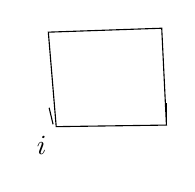
\begin{tikzpicture}\draw (0,0)--(1.4,.02)--(1.34,1.25)--(-.1,1.2)--cycle;\draw(-.04,.03)--(-.09,.24);\draw(1.4,.03)--(1.4,.3);\node[below left]at(0,0){$i$};\end{tikzpicture}}
\[
T_i\simeq\mathcal O\otimes_{\mathbb Z}\mathbb Z(\omega)
\]
et comparant, on trouve $L(\omega)=\mathbb Z$, donc en définitive
\[
\boxed{\widehat T_i\simeq\mathcal O(1)}\simeq\check F(\omega)
\]
\margin{où
\diagram{\begin{tikzcd}[ampersand replacement=\&, column sep=small]
0\arrow[r,no head]\&F\arrow[r,no head]\&V(J)_\Sigma\arrow[r]\&\underline{\mathcal O}_\Sigma(1)\arrow[d]\\
\&\&\&0
\end{tikzcd}}}
On trouve donc
\[
S\widehat P_I\overset{\mathrm{déf}}{=}\prod_{/\unsure{M_i|\widehat M}}\widehat P_i
\simeq\left(\check V^*(\mathcal O(1))\right)^{4}_{/\underbrace{\widehat M_{0,I}}_{\Sigma_I}}
\simeq V^*(\mathcal O(1))\mathbin{\wedge}_{G_m}G_m^I
\]
donc
\[
SP_I\simeq\left(V^*(\mathcal O(1))\mid\underbrace{M_{0,I}}_{\Sigma_I^*}\right)\mathbin{\wedge}_{G_m}G_m^I
\]
d'où (sur $\mathbb C$ maintenant, et dans le \unsure{contexte} analy.)
\[
S\mathcal T_{0,I}\simeq\Pi_1\left(V^*(\mathcal O(1))\mid\Sigma_I^*\right)\mathbin{\wedge}_{\mathbb Z}\mathbb Z^I
\]
\mspage{17}
